\documentclass[12pt, a4paper, oneside]{ctexart}
\usepackage{amsmath, amsthm, amssymb, bm, color, graphicx, geometry, mathrsfs,extarrows, braket, booktabs, array}
\usepackage[colorlinks,linkcolor=red,anchorcolor=blue,citecolor=blue,urlcolor=blue,menucolor=black]{hyperref}
\setmainfont{Times New Roman}  % 设置英文字体
\setsansfont{Calibri}
\setmonofont{Consolas}

\linespread{1.4}
%\geometry{left=2.54cm,right=2.54cm,top=3.18cm,bottom=3.18cm}
\geometry{left=1.84cm,right=1.84cm,top=2.18cm,bottom=2.18cm}
\newenvironment{problem}{\par\noindent\textbf{题目. }}{\bigskip\par}
\newenvironment{solution}{\par\noindent\textbf{解答. }}{\bigskip\par}
\newenvironment{note}{\par\noindent\textbf{注记. }}{\bigskip\par}

\everymath{\displaystyle} % 默认全部行间公式
\DeclareMathOperator*\uplim{\overline{lim}} % 定义上极限 \uplim_{}
\DeclareMathOperator*\lowlim{\underline{lim}} % 定义下极限 \lowlim_{}
\let\leq=\leqslant % 将全部leq变为leqslant
\let\geq=\geqslant % geq同理

% 一些宏定义
\def\bd{\boldsymbol}    % 加粗(向量) boldsymbol
\def\disp{\displaystyle}% 使用行间公式 displaystyle(默认)
\def\tsty{\textstyle}   % 使用行内公式 textstyle
\def\sign{\text{sign}}  % sign function
\def\wtd{\widetilde}    % 宽波浪线 widetilde
\def\R{\mathbb{R}}      % Real number
\def\C{\mathbb{C}}      % Complex number
\def\d{\mathrm{d}}      % differential operator
\def\e{\mathrm{e}}      % Euler's number
\def\i{\mathrm{i}}      % imaginary number
\def\re{\mathrm{Re\,}}    % Real part
\def\im{\mathrm{Im\,}}    % Imaginary part
\def\L{\mathcal{L}}     % Loss function
\def\wdh{\widehat}      % 宽帽子 widehat
\def\ol{\overline}      % 上横线 overline
\def\ul{\underline}     % 下横线 underline
\def\add{\vspace{1ex}}  % 增加行间距
\def\del{\vspace{-3.5ex}}  % 减少行间距

% 基本信息
\newcommand{\RQ}{\today} % 日期
\newcommand{\km}{经济博弈论} % 科目
\newcommand{\bj}{强基数学002} % 班级
\newcommand{\xm}{吴天阳} % 姓名
\newcommand{\xh}{2204210460} % 学号

\begin{document}

%\pagestyle{empty}
\pagestyle{plain}
\vspace*{-15ex}
\centerline{\begin{tabular}{*5{c}}
    \parbox[t]{0.25\linewidth}{\begin{center}\textbf{日期}\\ \large \textcolor{blue}{\RQ}\end{center}} 
    & \parbox[t]{0.2\linewidth}{\begin{center}\textbf{科目}\\ \large \textcolor{blue}{\km}\end{center}}
    & \parbox[t]{0.2\linewidth}{\begin{center}\textbf{班级}\\ \large \textcolor{blue}{\bj}\end{center}}
    & \parbox[t]{0.1\linewidth}{\begin{center}\textbf{姓名}\\ \large \textcolor{blue}{\xm}\end{center}}
    & \parbox[t]{0.15\linewidth}{\begin{center}\textbf{学号}\\ \large \textcolor{blue}{\xh}\end{center}} \\ \hline
\end{tabular}}
\vspace*{4ex}

% 正文部分
\paragraph{6.}假设买到劣质品的消费者中只有一半事后会发现商品的低质量并索赔, 那么有退款承诺的二手车交易模型的均衡会发生怎样的变化?
\begin{solution}
    设$P_h,P_l$为卖方的高价和低价, 索赔$V-W$, 则如果买方以高价买入差车, 有$\frac{1}{2}$的概率退款, 则卖方的得益为
    \begin{equation*}
        \frac{1}{2}(P_h+W-V)+\frac{1}{2}P_h = P_h+\frac{W-V}{2},
    \end{equation*}
    所以当$P_h+\frac{W-V}{2} < P_l$时, 不如差车卖低价合算, 由均衡策略, 与第5节的完美贝叶斯均衡相同.
\end{solution}\del
\paragraph{7.}若你正在考虑收购一家公司的一万股股票, 卖方的开价是$2$元/股. 根据经营情况的好坏, 该公司股票的价值对于你来说有$1$元/股和$5$元/股两种可能, 但只有卖方知道经营的真是好坏, 你所知道的只是两种情况各占$50\%$的可能性. 如果在公司经营情况不好时, 卖方让你无法识别真实情况的"包装"费用是五万元, 问你是否会接受卖方的价格买下这家公司? 如果上述"包装"费用只用五千元, 你会怎样选择?
\begin{solution}
    \begin{figure}[htbp]
        \centering
        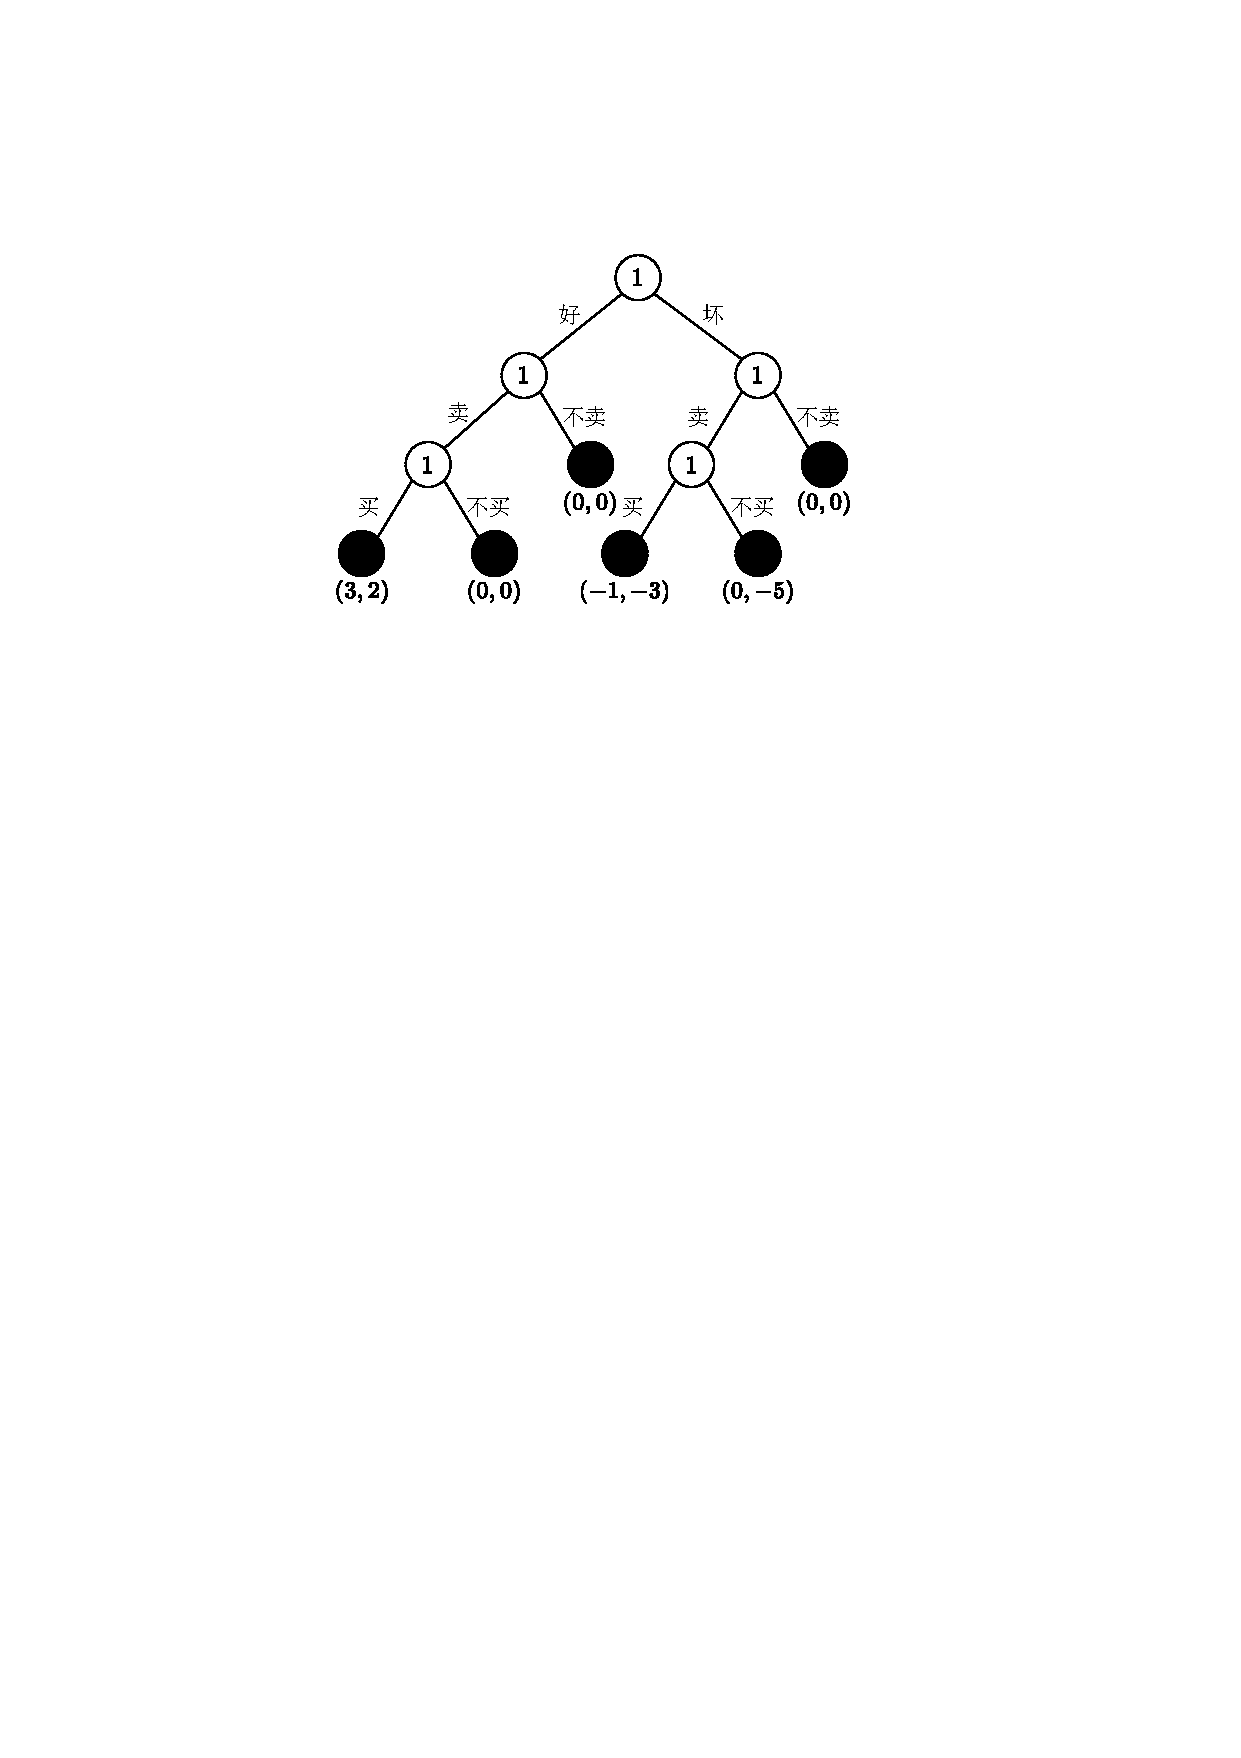
\includegraphics[scale=0.8]{5.7.pdf}
    \end{figure}
    根据上图不难看出, 当伪装费用为$5$万时, 公司经营情况坏的条件下, 不卖是卖的严格上策, 所以如果卖方进行卖出, 则我一定会选择买入.
    \begin{figure}[htbp]
        \centering
        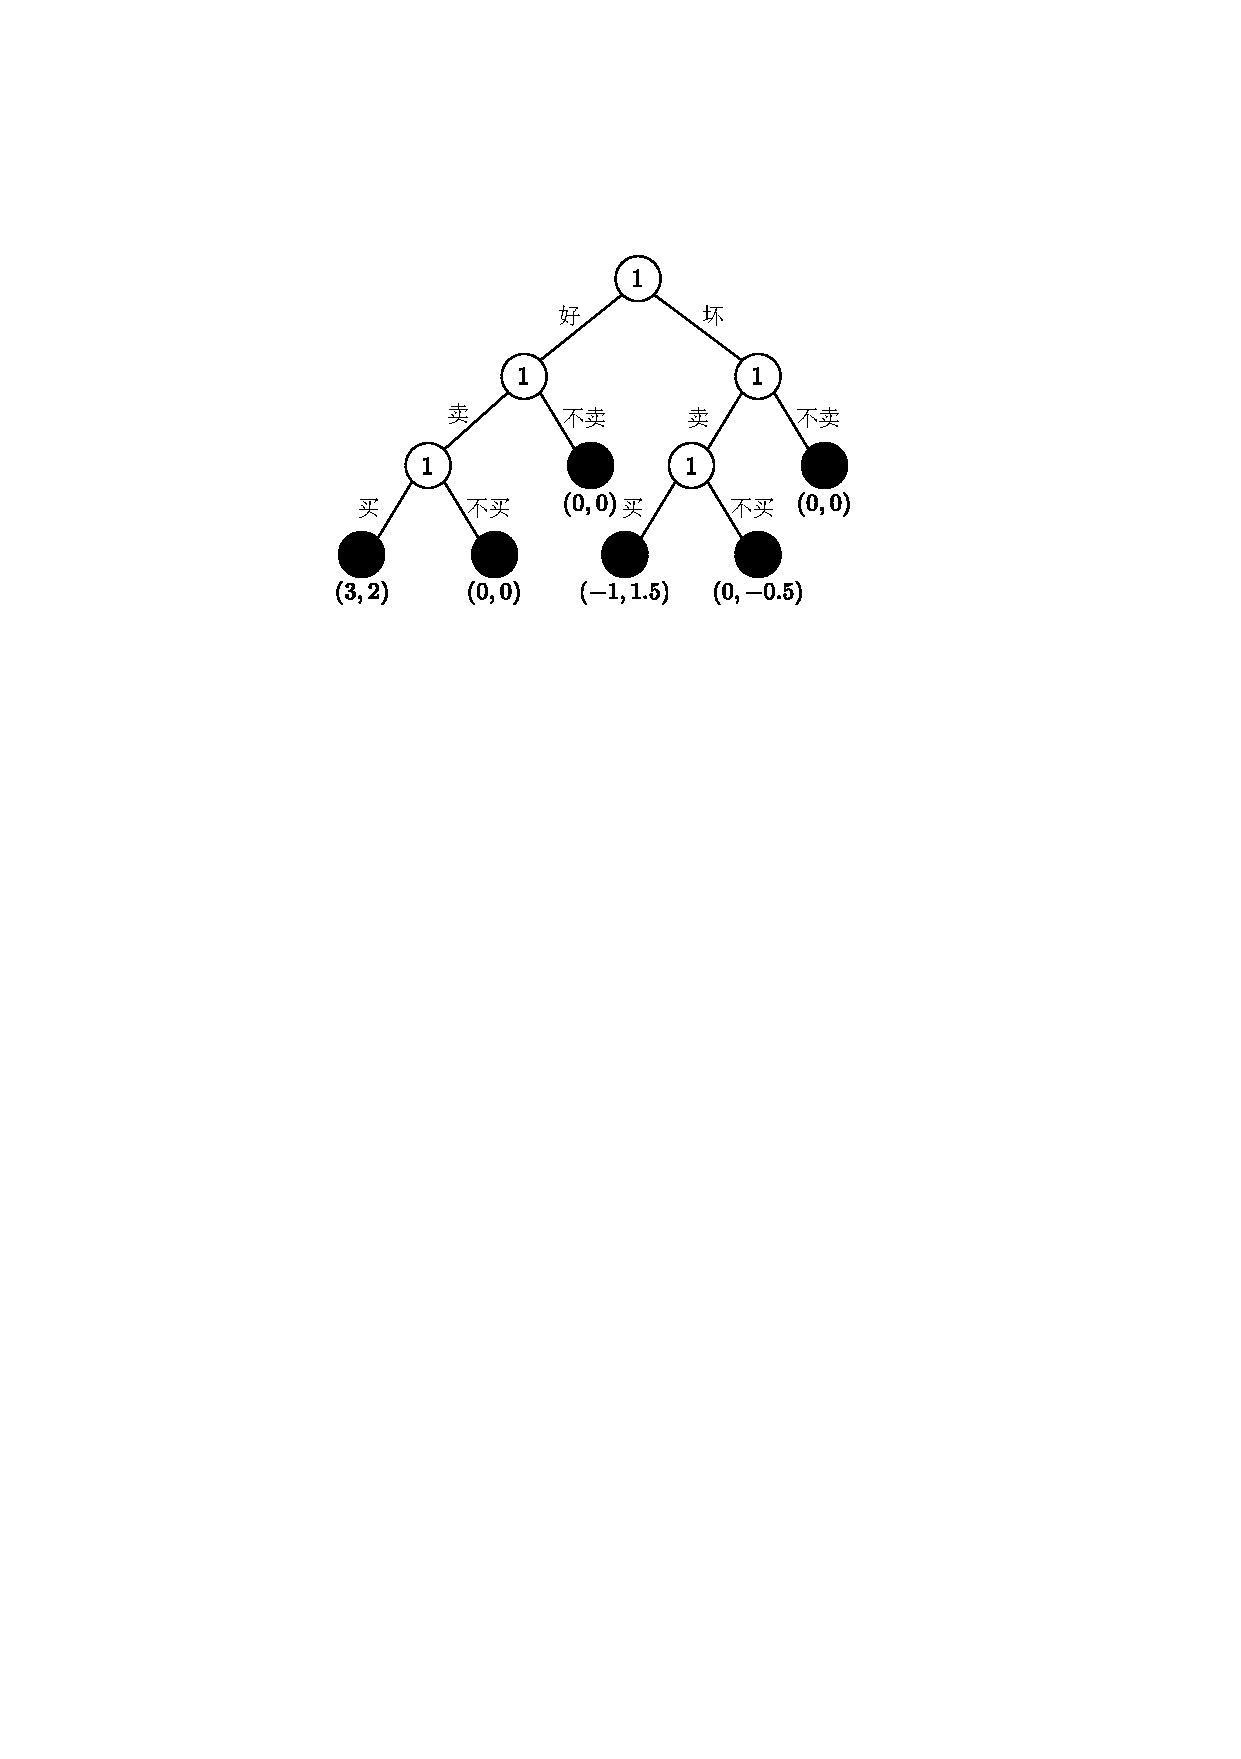
\includegraphics[scale=0.8]{5.7_1.pdf}
    \end{figure}

    如果伪装为用为$0.5$万时, 假设公司情况为坏的时候卖出的概率为$\frac{1}{2}$, 则根据贝叶斯法则
    \begin{equation*}
        p(g|s) = \frac{p(g)\cdot p(s|g)}{p(g)\cdot p(s|g)+p(b)\cdot p(s|b)} = \frac{0.5\times 1}{0.5\times 1+0.5\times 0.5} = \frac{2}{3},
    \end{equation*}
    所以我会以$\frac{2}{3}$概率判断他会卖出好情况下的公司, 若选择买入期望得益为$\frac{2}{3}\times 3 + \frac{1}{3}\times(-1) = \frac{5}{3}$, 不买的期望得益为 $0$, 所以我还是会选择买入.
\end{solution}
\paragraph{9.}证明本章最后一节最后一部分给出的策略组合在给定条件下构成一个市场成功类型的完美贝叶斯均衡. 并讨论 $0<P_h+W-V<P_l$时可能出现的变化.
\begin{proof}
    由于买方如论如何都不会亏本, 所以买方会买入所有的产品, 对于每个差商品加上索赔的获利, 都可以视为好商品, 所以该策略组合在给定条件下构成一个市场成功类型的完美贝叶斯均衡.

    当$0<P_h+W-V<P_l$时, 卖方可以可以通过卖出坏产品获得利润, 因此不能保证市场上的商品全部是好商品, 但是买方还是会买入所以有产品或有选择地买入产品, 所以变为市场部分成功或者接近失败类型.
\end{proof}

% 下面给一些功能的写法
\iffalse
% 图片模板
\centerline{
    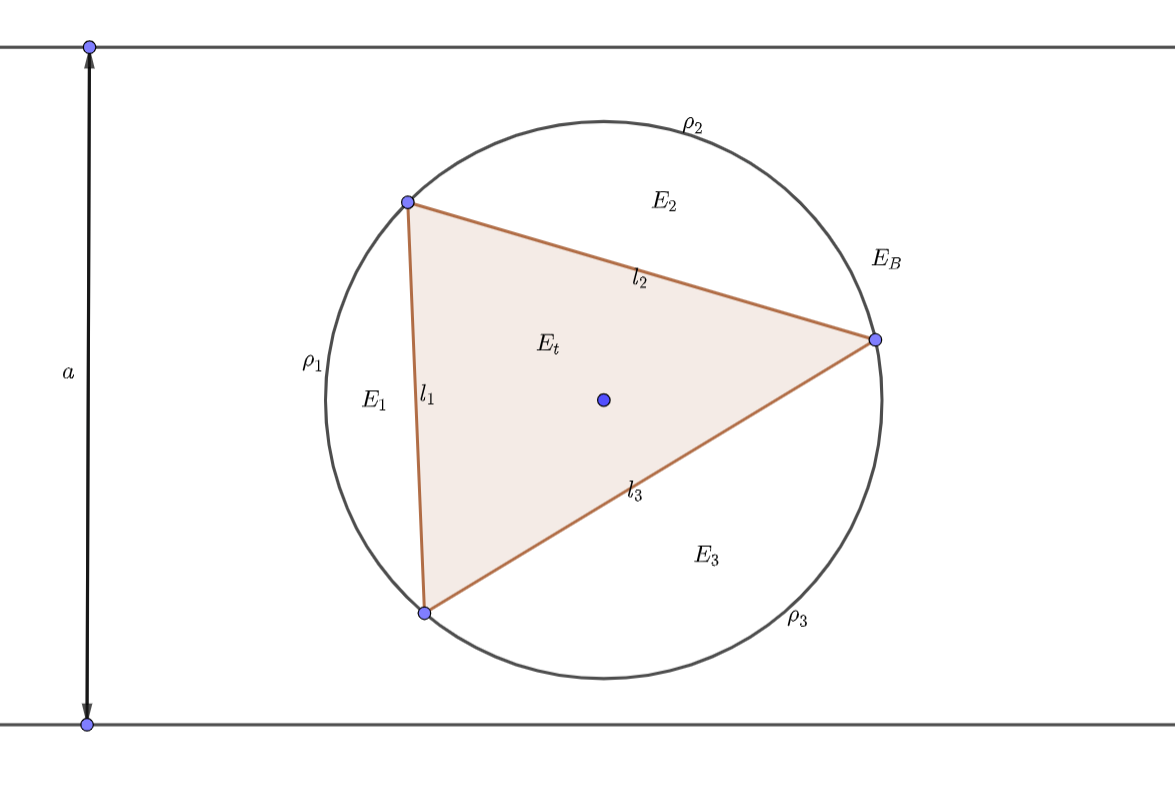
\includegraphics[width=0.8\textwidth]{figure.png}
}
% 表格模板
\renewcommand\arraystretch{0.8} % 设置表格高度为原来的0.8倍
\begin{table}[!htbp] % table标准
    \centering % 表格居中
    \begin{tabular}{p{1cm}<{\centering}p{1cm}<{\centering}p{3cm}<{\centering}p{5cm}<{\centering}} % 设置表格宽度
    %\begin{tabular}{cccc}
        \toprule
        $x_i$ & $f[x_1]$ & $f[x_i,x_{i+1}]$ & $f[x_i,x_{i+1},x_{i+2}]$ \\
        \midrule
        $x_0$ & $f(x_0)$ &                  &                          \\
        $x_0$ & $f(x_0)$ & $f'(x_0)$        &                          \\
        $x_0$ & $f(x_1)$ & $\frac{f(x_1)-f(x_0)}{x_1-x_0}$ & $\frac{f(x_1)-f(x_0)}{(x_1-x_0)^2}-\frac{f'(x_0)}{x_1-x_0}$\\
        \bottomrule
    \end{tabular}
\end{table}

\def\Log{\text{Log}} % 一个简单的宏定义
$\Log$ % 调用方法
\fi

\end{document}